\documentclass[svgnames,11pt]{beamer}
\input{/home/tof/Documents/Cozy/latex-include/preambule_commun.tex}
\input{/home/tof/Documents/Cozy/latex-include/preambule_beamer.tex}
%\usepackage{pgfpages} \setbeameroption{show notes on second screen=left}
\author[]{Christophe Viroulaud}
\title{Documentation}
\date{\framebox{\textbf{DonRep 10}}}
%\logo{}
\institute{Première - NSI}

\begin{document}
\begin{frame}
\titlepage
\end{frame}
\begin{frame}[fragile]
    \frametitle{}

    Python est un langage de haut niveau c'est à dire qu'il met à disposition des outils optimisés facilitant la vie du développeur. 
    \begin{center}
    \begin{lstlisting}[language=Python , basicstyle=\ttfamily\small, xleftmargin=2em, xrightmargin=2em]
>>> tab = [1, 4, 2, 8]
>>> len(tab)
4
\end{lstlisting}
    \captionof{code}{Taille d'une liste}
    \label{CODE}
    \end{center}

\end{frame}
\begin{frame}
    \frametitle{}

    \begin{framed}
        \centering Comment utiliser efficacement un langage informatique?
    \end{framed}

\end{frame}
\section{Découvrir la documentation}
\begin{frame}
    \frametitle{Découvrir la documentation}
\begin{aretenir}[]
Chaque langage informatique s'accompagne d'une documentation. Il n'est pas possible de la connaître par cœur. Il faut cependant savoir l'utiliser.
\end{aretenir}
\begin{activite}
\begin{enumerate}
    \item Dans un moteur de recherche, entrer les mots-clés \textbf{\texttt{documentation python}}.
    \item Dans les menus déroulants, choisir la langue et la version de Python.
    \item Chercher les fonctionnalités des tableaux (appelés \textbf{\texttt{list}} en Python).
\end{enumerate}
\end{activite}
    

\end{frame}
\begin{frame}
    \frametitle{Correction}

    \begin{center}
        \url{https://docs.python.org/fr/3/tutorial/datastructures.html}
        \end{center}

\end{frame}
\section{Comprendre la documentation}
\begin{frame}
    \frametitle{Comprendre la documentation}

\begin{aretenir}[]
    La documentation donne le nom de la méthode et les \emph{paramètres} éventuels.
\end{aretenir}
\begin{framed}
    \texttt{\textbf{list.pop([i])}}\\
Enlève de la liste l'élément situé à la position indiquée et le renvoie en valeur de retour. Si aucune position n'est spécifiée, a.pop() enlève et renvoie le dernier élément de la liste.
\end{framed}
\end{frame}
\begin{frame}[fragile]
    \frametitle{}

    \begin{activite}
    \begin{enumerate}
        \item Construire le tableau \textbf{\texttt{tab}}
\begin{lstlisting}[language=Python , basicstyle=\ttfamily\small, xleftmargin=2em, xrightmargin=2em]
tab = [3, 18, 8, 1, 9, 10]
\end{lstlisting}
        \item Extraire le dernier élément de la liste et l'affecter à une variable \textbf{\texttt{dernier}}.
        \item Extraire le troisième élément et l'affecter à une variable \textbf{\texttt{troisième}}.
    \end{enumerate}
    \end{activite}

\end{frame}
\begin{frame}[fragile]
    \frametitle{Correction}

    \begin{lstlisting}[language=Python , basicstyle=\ttfamily\small, xleftmargin=2em, xrightmargin=2em]
tab = [3, 18, 8, 1, 9, 10]
print(tab)

dernier = tab.pop()
print(tab)

troisieme = tab.pop(2)
print(tab)
\end{lstlisting}    

\end{frame}
\begin{frame}
    \frametitle{}

    \begin{activite}
    \begin{enumerate}
        \item Construire un tableau \textbf{\texttt{tab}} vide.
        \item Dans la documentation, trouver la méthode permettant d'ajouter un élément à la fin du tableau.
        \item Ajouter 5 entiers dans le tableau.
    \end{enumerate}
    \end{activite}

\end{frame}
\begin{frame}[fragile]
    \frametitle{Correction}
    \begin{framed}
        \texttt{\textbf{list.append(x)}}\\
        Ajoute un élément à la fin de la liste. Équivalent à \texttt{\textbf{a[len(a):] = [x]}}.
    \end{framed}

\begin{lstlisting}[language=Python , basicstyle=\ttfamily\small, xleftmargin=2em, xrightmargin=2em]
tab = []
tab.append(4)
tab.append(12)
tab.append(9)
tab.append(1)
tab.append(10)
\end{lstlisting}

\end{frame}
\begin{frame}[fragile]
    \frametitle{}

    \begin{center}
\begin{lstlisting}[language=Python , basicstyle=\ttfamily\small, xleftmargin=2em, xrightmargin=2em]
from random import randint

tab = []
for i in range(5):
    tab.append(randint(1, 100))
\end{lstlisting}
\captionof{code}{Ajout de 5 entiers aléatoires dans le tableau}
\label{CODE}
\end{center}    

\end{frame}
\section{Avantage d'un langage de haut-niveau}
\begin{frame}
    \frametitle{Avantage d'un langage de haut-niveau}

    
    \begin{center}
        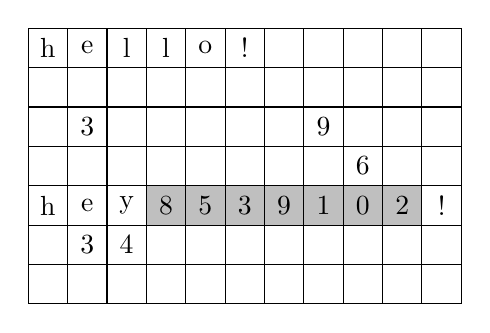
\begin{tikzpicture}[scale=0.5]
            \fill[gray!50] (3,2) rectangle (10,3);
            \draw (0,0) grid (11,7);

            \draw (0.5,2.5) node{h};
            \draw (1.5,2.5) node{e};
            \draw (2.5,2.5) node{y};

            \draw (0.5,6.5) node{h};
            \draw (1.5,6.5) node{e};
            \draw (2.5,6.5) node{l};
            \draw (3.5,6.5) node{l};
            \draw (4.5,6.5) node{o};
            \draw (5.5,6.5) node{!};

            \draw (10.5,2.5) node{!};
            \draw (7.5,4.5) node{9};
            \draw (8.5,3.5) node{6};
            \draw (1.5,4.5) node{3};
            \draw (2.5,1.5) node{4};
            \draw (1.5,1.5) node{3};

            \foreach \x/\y in {3/8,4/5,5/3,6/9,7/1,8/0,9/2}
                {\draw (\x+0.5,2.5) node{\y};}
        \end{tikzpicture}
        \captionof{figure}{\centering En théorie un tableau est enregistré dans un espace libre en mémoire.}
        \label{IMG}
    \end{center}
    \begin{center}
        Que se passe-t-il quand on veut agrandir le tableau?
    \end{center}
\end{frame}
\begin{frame}
    \frametitle{}

    \begin{center}
        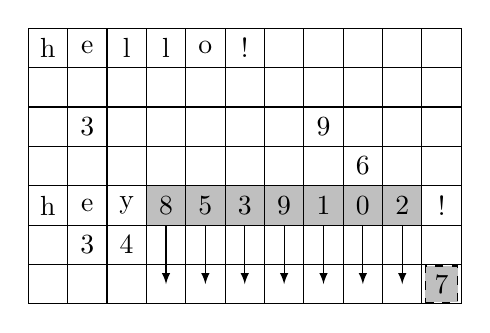
\begin{tikzpicture}[scale=0.5]
            \fill[gray!50] (3,2) rectangle (10,3);
            \draw (0,0) grid (11,7);

            \draw (0.5,2.5) node{h};
            \draw (1.5,2.5) node{e};
            \draw (2.5,2.5) node{y};

            \draw (0.5,6.5) node{h};
            \draw (1.5,6.5) node{e};
            \draw (2.5,6.5) node{l};
            \draw (3.5,6.5) node{l};
            \draw (4.5,6.5) node{o};
            \draw (5.5,6.5) node{!};

            \draw (10.5,2.5) node{!};
            \draw (7.5,4.5) node{9};
            \draw (8.5,3.5) node{6};
            \draw (1.5,4.5) node{3};
            \draw (2.5,1.5) node{4};
            \draw (1.5,1.5) node{3};

            \foreach \x/\y in {3/8,4/5,5/3,6/9,7/1,8/0,9/2}
                {\draw (\x+0.5,2.5) node{\y};
                    \draw[->,>=latex] (\x+.5,2) -- (\x+.5,.5);
                }
            \node[draw,dashed,fill=gray!50] at(10.5,.5) {7};
        \end{tikzpicture}
        \captionof{figure}{\centering Pour ajouter un élément au tableau il faut ici recopier entièrement ce-dernier dans un espace libre.}
        \label{IMG}
    \end{center}
\begin{aretenir}[]
L'ajout d'un élément à un tableau peut avoir un coût en temps d'exécution important.
\end{aretenir}
\end{frame}
\begin{frame}
    \frametitle{}

    \begin{aretenir}[]
    Par des mécanismes complexes, Python (\textbf{\texttt{list}}) minimisent les coûts d'exécution lors de l'agrandissement d'un tableau. \\Dans la mesure du possible on essaiera de privilégier des tableaux de taille fixe. 
    \end{aretenir}

\end{frame}
\end{document}